The software design was mainly guided by the provided format of the raw data. Which was from a few different sources, as different people were working with different data at the Hospital, and they did not have a unified collection. Thus the following documentation of the software design will be structured going from the raw data, to the preprocessed data, and then the model itself.

\section{Raw Data}

The raw data is scattered amongst many files, are registered in different spaces, does not have masks applied, along with other challenges detailed in \reflink{sec:preproc}{Section}.

\begin{figure}[H]
\centering
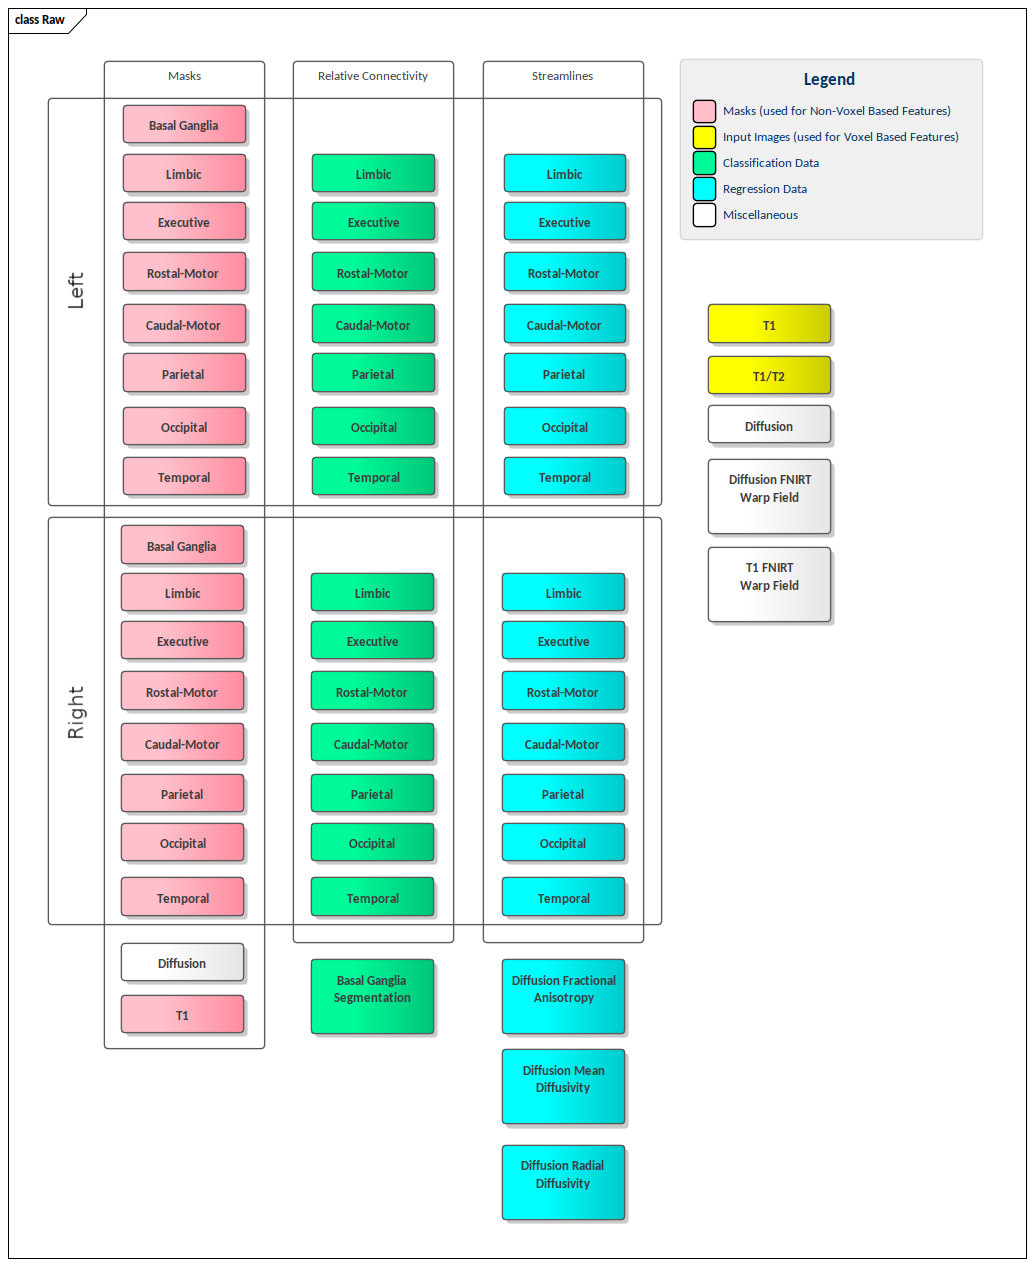
\includegraphics[width=0.7\textwidth]{DataRaw}
\caption{Files: Raw}
\end{figure}

The following class diagram documentations are detailed abstractions of the actual source code, as \ac{UML} is not completely Python compliant. Before moving on, the following simple data types are used in the \ac{UML} diagrams:

\begin{figure}[H]
\centering
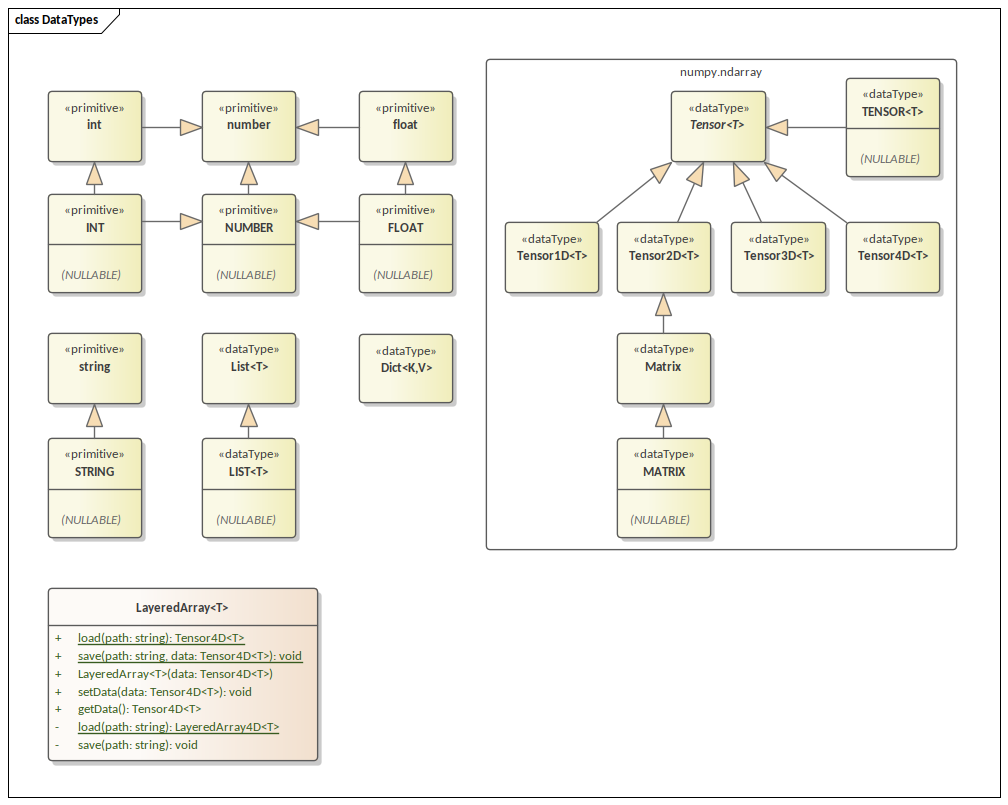
\includegraphics[width=0.7\textwidth]{ClassDataTypes}
\caption{Class Diagram: Data Types}
\end{figure}

There is one odd one out in this diagram, that being the LayeredArray, which is more than a simple data type or primitive. This class is a simple space efficient data structure of a 4D tensor.\par
Storing some of the data provided can be highly inefficient by storing the raw tensor. Ultimately the design aims to collect the scattered data from multiple files, into clean logical groups, for example all the cortical target masks into a single 4D tensor where the 4th dimension is reserved for the multiple targets. But this poses a greatly inefficient way of storing the data, as each target region only takes up a small portion of the entire space. The idea behind the LayeredArray class, it stores the 4D tensor as a list of 3D tensors, each cropped down to their effective space where there are non-zero voxels. This also requires an additional list of 3D vectors to store each layer's origin, and where to paste it in the original space.\par
This solution offers a very efficient way of storing data for this use case, as the raw storage solution for the cortical targets were around 50MBs, and this cuts it down to 3MBs. This is even more drastic for the relative connectivity, which is more than a simple boolean mask and proportionally takes up even less space of the entire brain; in which's case it was cut down from 110MBs to 0.5MBs, reducing the disk requirement by several magnitudes.\par
The original \ac{NIfTI} format also does a very good job at storing data efficiently, but this solution provides a more lower level control over the way of storing the data. This is beneficial as the data are stored in numpy format, making it easier to ignore certain data type safety checks, data type conversions, and leaving behind the \ac{NIfTI} format's additional complexity of the orientation, transformation, and many more nuances that are part of the \ac{NIfTI} header.\par
This has the undoubted drawback of not being able to use \ac{FSL} tools natively on our datatypes, such as fsleyes for simply viewing a record. But thanks to the opensource nature of the \ac{FSL} suite, with a few additional lines of code, support can be added for our datatypes (included in \reflink{apx:source}{Appendix}).

\begin{figure}[H]
\centering
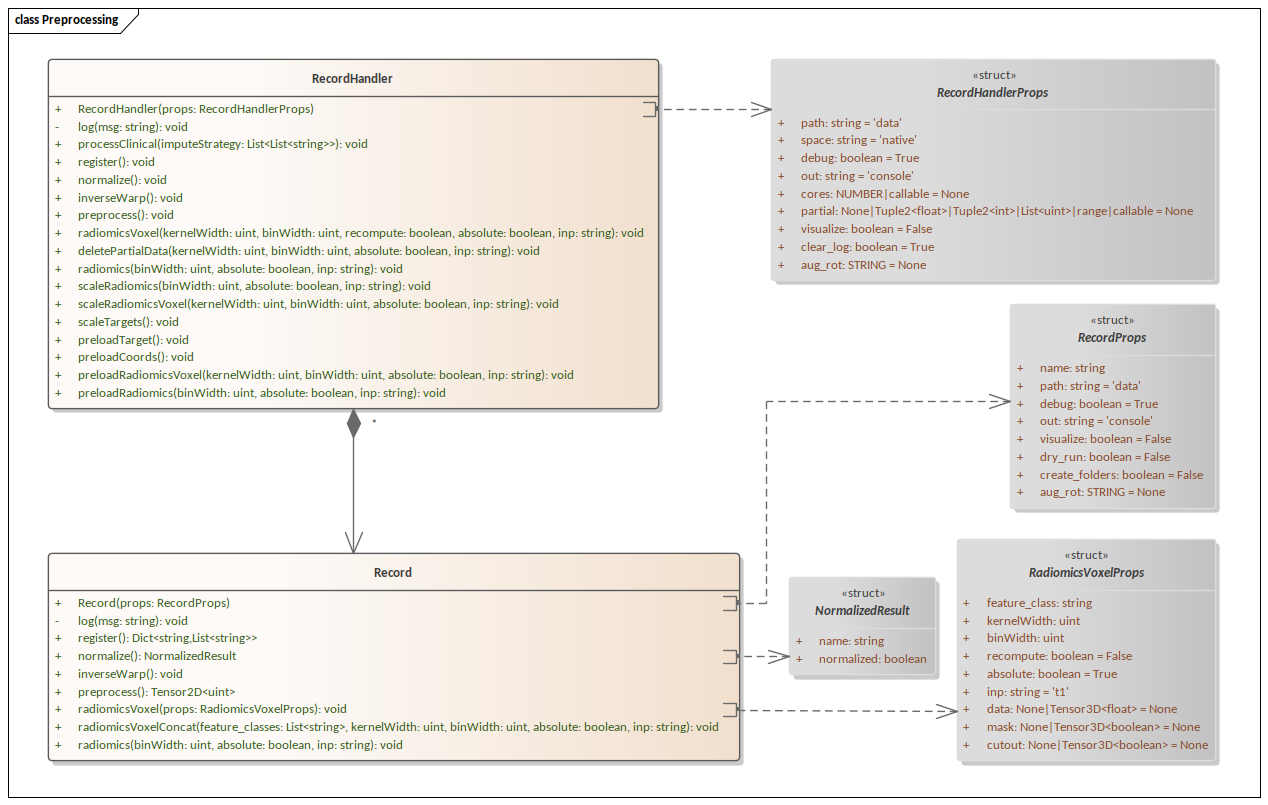
\includegraphics[width=0.7\textwidth]{ClassPreprocessing}
\caption{Class Diagram: Preprocessing}
\end{figure}

The class diagram above contains the two classes responsible for the preprocessing of the data. The RecordHandler being the controller itself that handles the high level operations on a collection of records. And the records handling the low level computations on the data itself.

\section{Common Functions}

There are set of static common functions, which give the low level backbone of the entire project. They are grouped into two categories, util and visual. Where the prior one contains everything from simple data type castings, external \ac{FSL} library system calls, to computing radiomics, and more. And the latter one is a collection of functions for visualizing data.

\begin{figure}[H]
\centering
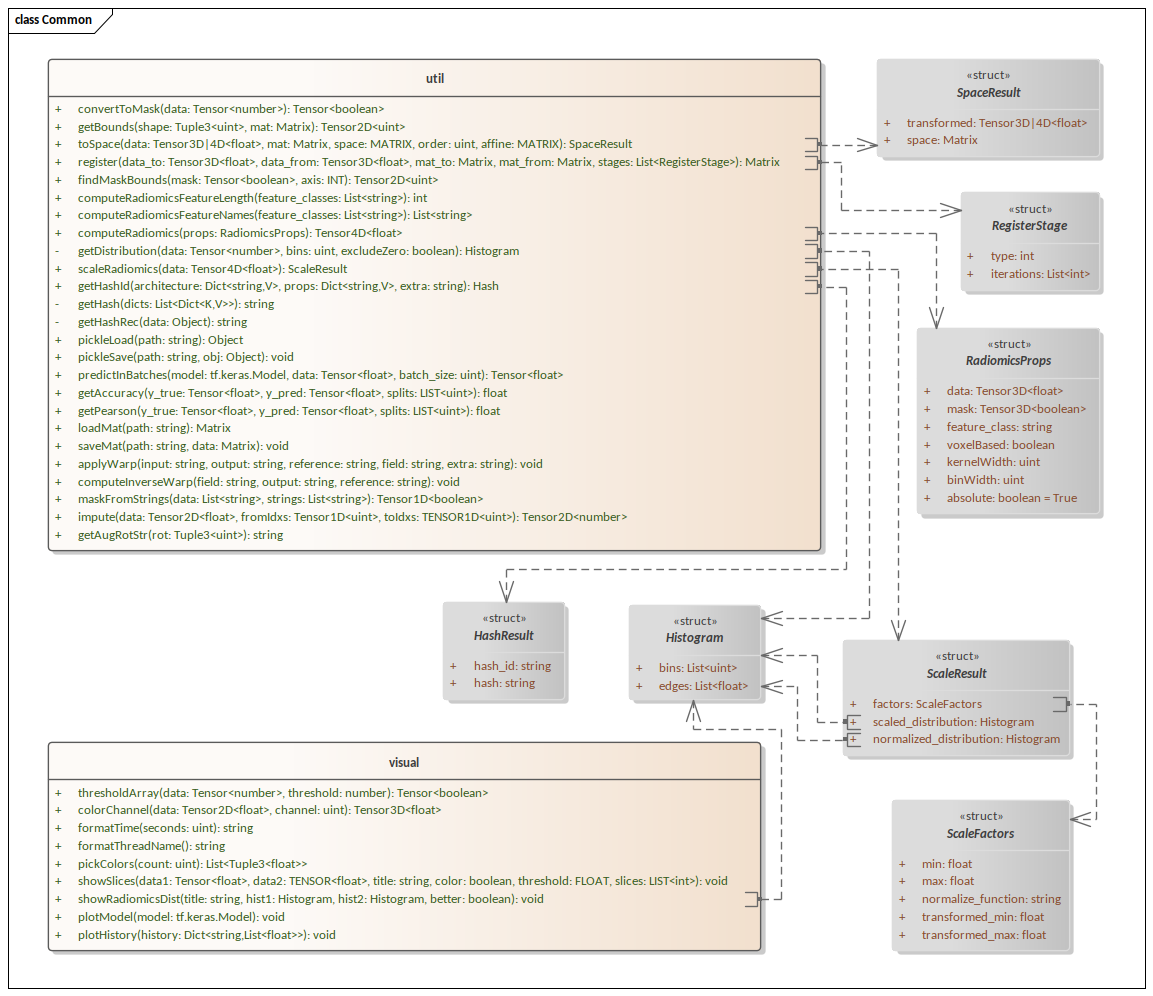
\includegraphics[width=0.7\textwidth]{ClassCommon}
\caption{Class Diagram: Common}
\end{figure}

\section{Preprocessed Data}

Preprocessing the data are composed from the next few high level operations done by the RecordHandler:
\begin{enumerate}
  \item Register some records (not needed for most of them)
  \item Compute all normalized records
  \item Compute the inverse \ac{FNIRT} warp field (they weren't provided)
  \item Convert native records into our numpy format (compute the affine transformations, merge different sources, etc.)
  \item Compute scaling factors across all native records
  \item Preload native records
  \item Convert normalized records into our numpy format
  \item Compute scaling factors across all normalized records
  \item Preload normalized records
  \item Construct normalized coordinate maps
  \item Warp normalized coordinate maps into native space
  \item Scale and preload coordinate maps
  \item Impute clinical data
\end{enumerate}

After preprocessing, the next set of logical grouping and files are left:

\begin{figure}[H]
\centering
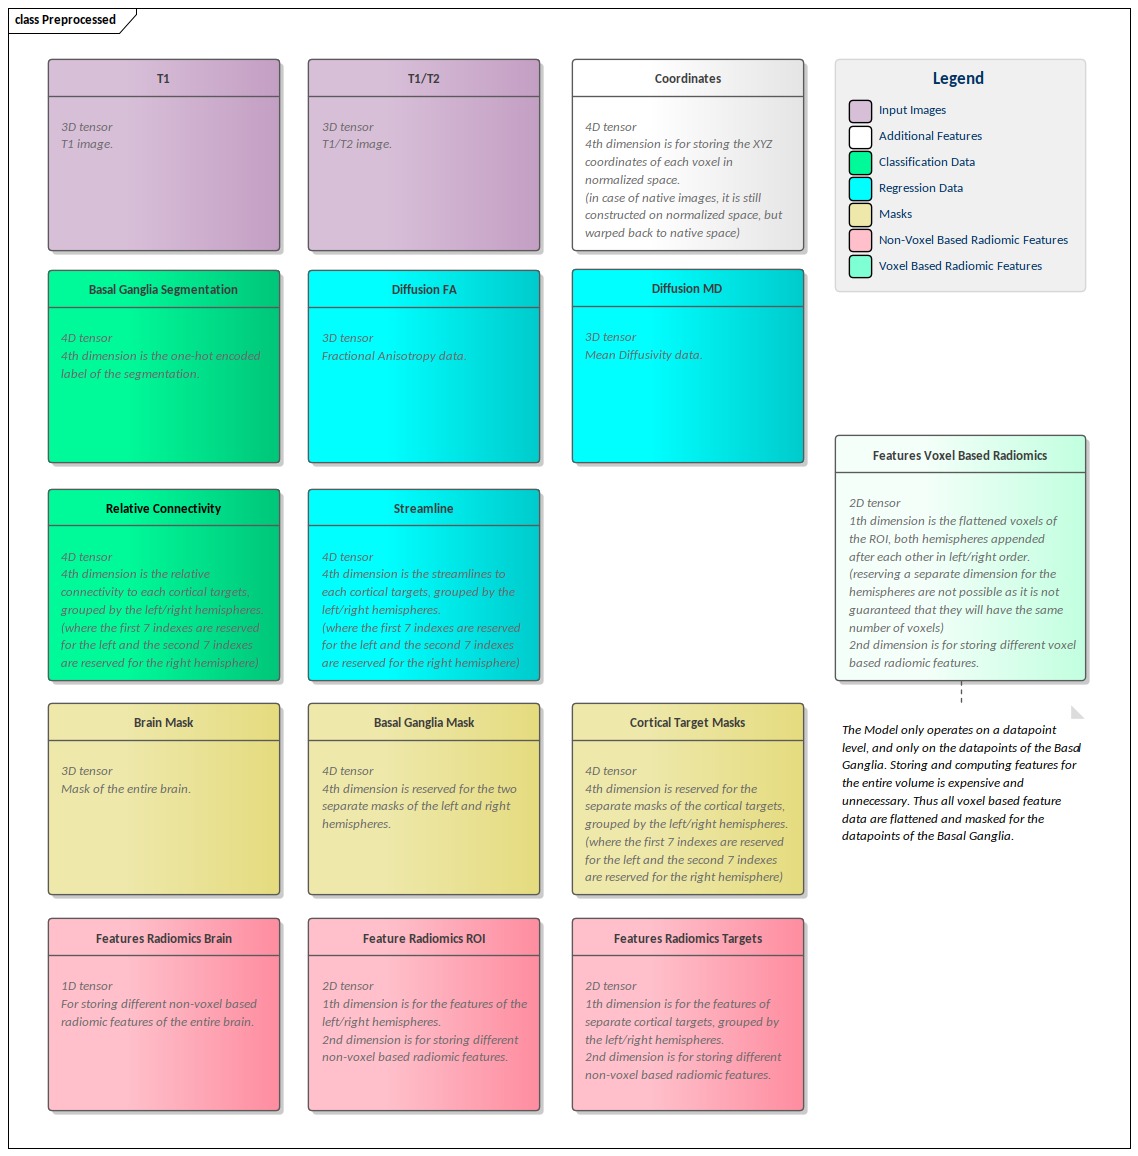
\includegraphics[width=0.7\textwidth]{DataPreprocessed}
\caption{Files: Preprocessed}
\end{figure}

However, this project focuses on only the voxels inside the Basal Ganglia, meaning the model on a datapoint level is never going to operate outside of that region. Thus, the voxels of the \ac{ROI} can be 'preloaded' so the DataGenerator class, used for feeding the model data, can very efficiently only load the datapoints that it needs. Furthermore this can also be applied when computing the radiomic features, as it only needs to be computed for the \ac{ROI}.




